\documentclass[Thesis.tex]{subfiles}
\begin{document}
\chapter{Simulation and results}

The \gls{ROS} node built for \gls{AMCL6D} also includes a simple tool to simulate a robot pose. This tool was used to simulate and test the algorithm. The performance of the algorithm it was tested on different maps or with different resolutions. To assure accuracy, for each map there was a random but arbitrary sequence of motions defined which was repeated for each trial. The simulated camera for the ray tracing always had aperture angles of $90^\circ$ (horizontal) and $60^\circ$ (vertical).

\section{Performance in different maps}
The performance is measured by taking the distance between the simulated real pose and the best hypothesis after each time step. Hence lower values mean better results.

\subsection*{Elevator doors}

\begin{figure}[h]\centering
\begin{tabularx}{\textwidth}{XlrrX}
  &\multicolumn{2}{c}{\small\bf Map and test properties} & \multirow{11}{*}{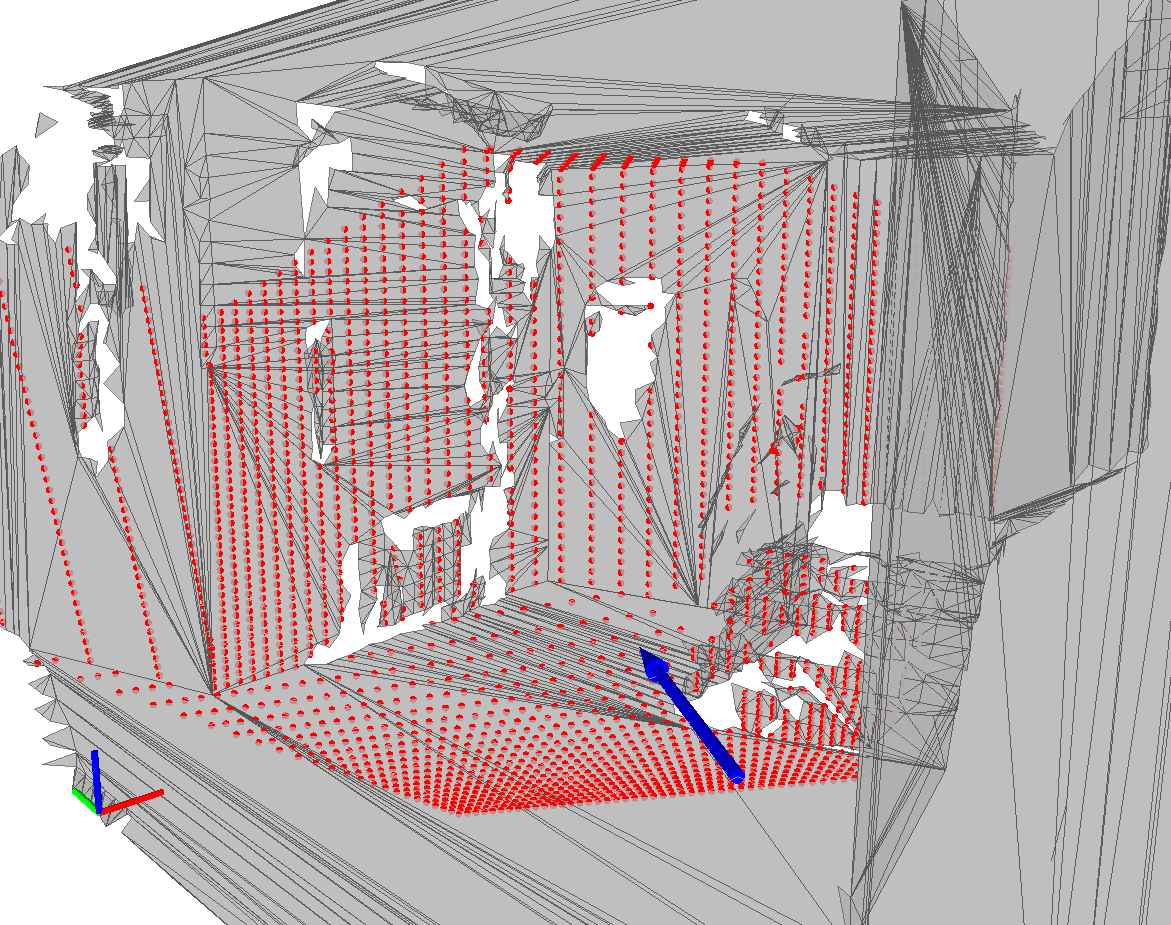
\includegraphics[width=.5\columnwidth]{pics/example_raytrace}}&\\
	&Vertex count & 3,774 &\\
  &Face count  & 3,924 &\\
  &Iterations  & 100 &\\
  &Resolution  & 65x45 &\\
  &&&\\
  &&&\\
  &&&\\
  &&&\\
  &&&\\
  &&&\\
\end{tabularx}
\caption{Map and test properties: Elevator doors}
\label{fig:elvmapprop}
\end{figure}

The elevator doors map is open on one side and has lots of holes. It is smaller in size than the office map, but has more vertices and faces.

The results below show that the algorithm is not capable of localizing the robot within 100 iterations. However it is interesting that the algorithm decreases the distance steadily during the first half of each experiment but after about 50 iterations it spikes far away and has problems to recover.

\begin{center}
\begin{tikzpicture}
\begin{axis}[xlabel={Iterations}, ylabel={Distance},axis lines=left,width=.8\textwidth,height=.5\textwidth,legend entries={mean values}]
\addplot[thin, orange]        table [x=iter, y=avg, col sep=comma]  {data/elvavg.csv};
\draw[-,red] (axis cs:0,5.05) -- (axis cs:100,5.05);
\addplot[ultra thin, gray!90] table [x=iter, y=dist, col sep=comma] {data/elv3.txt};
\addplot[ultra thin, gray!80] table [x=iter, y=dist, col sep=comma] {data/elv4.txt};
\addplot[ultra thin, gray!70] table [x=iter, y=dist, col sep=comma] {data/elv5.txt};
\addplot[ultra thin, gray!60] table [x=iter, y=dist, col sep=comma] {data/elv6.txt};
\addplot[ultra thin, gray!50] table [x=iter, y=dist, col sep=comma] {data/elv7.txt};
\end{axis}
\end{tikzpicture}
\end{center}

\subsection{Office corridor}
\begin{figure}[h]\centering
\begin{tabularx}{\textwidth}{XlrrX}
  &\multicolumn{2}{c}{\small\bf Map and test properties} & \multirow{11}{*}{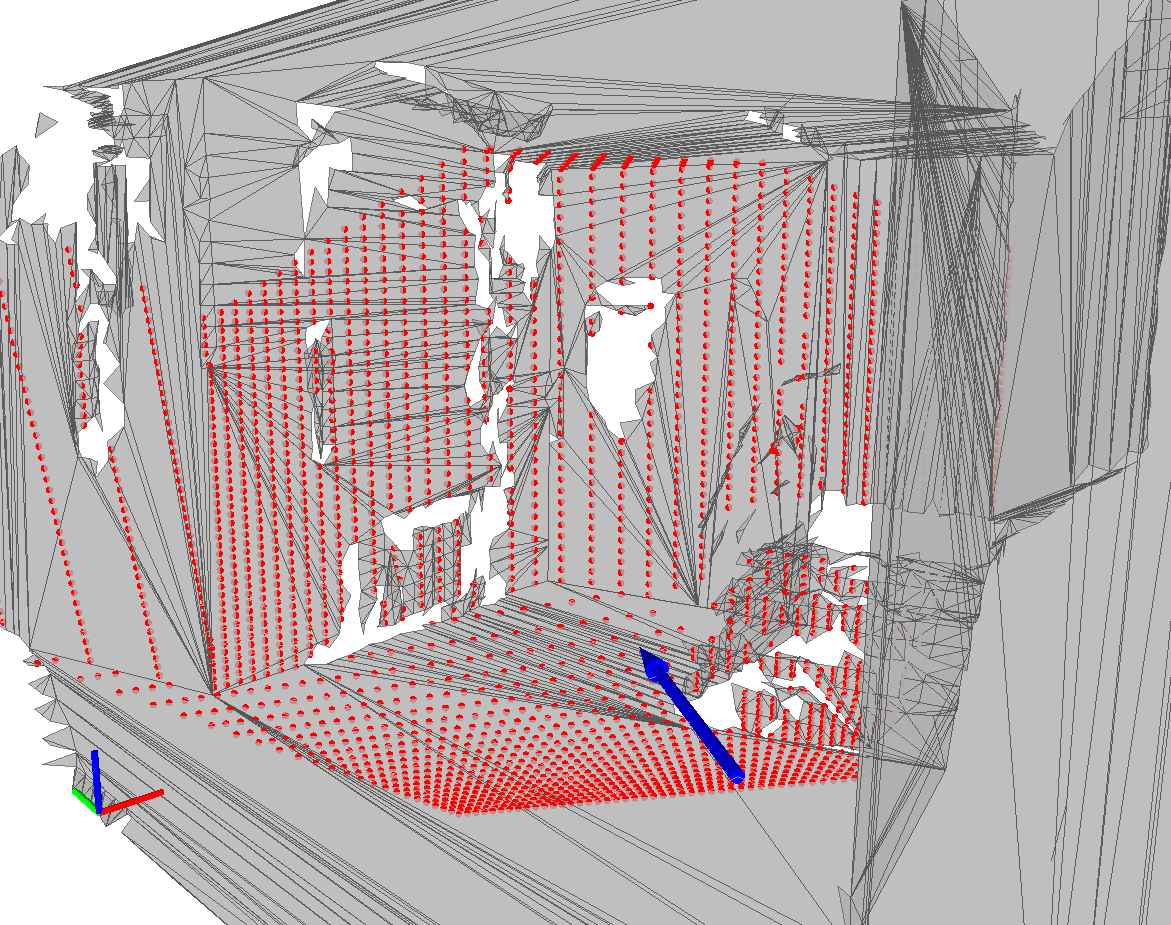
\includegraphics[width=.5\columnwidth]{pics/example_raytrace}}&\\
	&Vertex count & 1,018 &\\
  &Face count  & 857 &\\
  &Iterations  & 100 &\\
  &Resolution  & 65x45 &\\
  &&&\\
  &&&\\
  &&&\\
  &&&\\
  &&&\\
  &&&\\
\end{tabularx}
\caption{Map and test properties: Office corridor}
\label{fig:offmapprop}
\end{figure}


\section{Resolution of ray tracer}
To see how much impact the resolution of the sensor model has and if there are better resolutions, tests in the same elevator doors map (\figRef{fig:evlmapprop}) with different resolutions of 100x80 (2 runs), 65x45 (5), 30x20 (5) were compared.

The mean results are plotted below. As one can see, all resolutions perform similar.
\begin{center}
\begin{tikzpicture}
\begin{axis}[xlabel={Iterations}, ylabel={Distance},axis lines=left,width=.8\textwidth,height=.5\textwidth, legend style={at={(.5,1)},anchor=north}]
\addplot[red]    table [x=iter, y=avg, col sep=comma] {data/elvsavg.csv};
\addlegendentry{30x20}
\addplot[blue] table [x=iter, y=avg, col sep=comma] {data/elvavg.csv};
\addlegendentry{65x45}
\addplot[olive]  table [x=iter, y=avg, col sep=comma] {data/elvhavg.csv};
\addlegendentry{100x80}
\end{axis}
\end{tikzpicture}
\end{center}



\section{Ray tracing speed}
During the tests the time of the ray tracer was tracked to find out its portion of time used in the algorithm.
The results show that the ray tracer most of the node's running time consumes and that it is a huge bottleneck.

\begin{center}\small
\noindent\begin{tabular}{r|lc|rr|l}
\bf Run & \bf Map        & \bf Resolution & \bf Total time (s) & \bf RT time (s) & \bf \nicefrac{RT}{Total} (\%) \\ \toprule
1&Elevator&65x45&2139&2037&95.23\\
2&Elevator&65x45&2191&2085&95.16\\
3&Elevator&65x45&1867&1766&94.59\\
4&Elevator&65x45&2250&2146&95.38\\
5&Elevator&65x45&2084&1979&94.96\\
6&Elevator&65x45&2229&2124&95.29\\
7&Elevator&65x45&1944&1840&94.65\\
8&Elevator&30x20&481&457&95.01\\
9&Elevator&30x20&430&407&94.65\\
10&Elevator&30x20&528&504&95.45\\
11&Elevator&30x20&407&384&94.35\\
12&Elevator&30x20&464&443&95.47\\
13&Elevator&100x80&6166&5890&95.52\\
14&Elevator&100x80&6012&5730&95.31\\
15&Office&65x45&787&745&94.66\\
16&Office&65x45&764&722&94.50\\
17&Office&65x45&803&762&94.89\\
18&Office&65x45&786&737&93.77\\
19&Office&65x45&827&786&95.04\\
\bottomrule
\end{tabular}\end{center}





\end{document}
